\section*{ÔN TẬP KIỂM TRA CUỐI KÌ 2 - ĐỀ 02}
\setcounter{ex}{0}\setcounter{bt}{0}
\noindent{\bf\fontfamily{qag}\selectfont\color{violet}A. PHẦN TRẮC NGHIỆM}
\Opensolutionfile{ans}[ans/ansBTTeXCK22]
%Câu 1
\begin{ex}
 Số tập con gồm đúng $2$ phần tử của tập hợp gồm $7$ phần tử bằng
\choice
{$A_7^2$}
{$2^7$}
{\True $C_7^2$}
{$2^7-1$}
\loigiai{ Mỗi tập con gồm $2$ phần tử lấy từ tập hợp gồm $7$ phần tử là một tổ hợp chập $2$ của $7$.\\
Do đó, số tập con cần tìm là $C_7^2$
}
\end{ex}
%Câu 2
\begin{ex}
 Từ các chữ số 1,2,3,4,5,6. Có thể lập được bao nhiêu số có $2$ chữ số khác nhau?
\choice
{$36$}
{\True $30$}
{$15$}
{$12$}
\loigiai{ Mỗi số có hai chữ số khác nhau lập được từ các chữ số 1,2,3,4,5,6 là một chỉnh hợp chập $2$ của $6$ phần tử. Nên số các số lập được là $A_6^2=30$
}
\end{ex}
%Câu 3
\begin{ex}
 Có bao nhiêu cách trao $5$ phần quà khác nhau cho $5$ học sinh (mỗi học sinh một phần quà)?
\choice
{10}
{24}
{5}
{\True 120}
\loigiai{ Mỗi cách trao $5$ phần quà khác nhau cho $5$ học sinh là một hoán vị của 5 phần tử.\\
Vậy có $5!=120$ cách
}
\end{ex}
%Câu 4
\begin{ex}
 Khai triển nhị thức $(2x+3)^5$ có bao nhiêu số hạng?
\choice
{\True $6$}
{$7$}
{$9$}
{${5^{5}}$}
\loigiai{ 
Khai triển nhị thức $(a+b)^5$ thì có $6$ số hạng.
}
\end{ex}
%Câu 5
\begin{ex}
Viết khai triển theo công thức nhị thức Newton ${{(x+1)}^5}$.
\choice
{\True $x^5+5x^4+10x^3+10x^2+5x+1$}
{$x^5-5x^4-10x^3+10x^2-5x+1$}
{$x^5-5x^4+10x^3-10x^2+5x-1$}
{$5x^5+10x^4+10x^3+5x^2+5x+1$}
\loigiai{ Ta có: $(x+1)^5=C_5^0 x^5+C_5^1x^4+C_5^2x^3+C_5^3x^2+C_5^4x+C_5^5=x^5+5x^4+10x^3+10x^2+5x+1$
}
\end{ex}
%Câu 6
\begin{ex}
Số quy tròn của của $20182020$ đến hàng trăm là:
\choice
{\True $20182000$}
{$20180000$}
{$20182100$}
{$20182020$}
\loigiai{ Số quy tròn của của $20182020$ đến hàng trăm là: $20182000$
}
\end{ex}
%Câu 7
\begin{ex}
 Điều tra số học sinh của $30$ lớp học, ta được bảng số liệu như sau: 
$35$ $39$ $39$ $40$ $40$ $41$ $41$ $41$ $41$ $44$ $44$ $45$ $45$ $45$ $46$
$48$ $48$ $48$ $48$ $49$ $49$ $49$ $49$ $49$ $49$ $50$ $50$ $50$ $50$ $51$
 Số trung vị của bảng nói trên là:
\choice
{$46$}
{$48$}
{$45$}
{\True $47$}
\loigiai{
Ta có: $N=30$ là số chẵn. Số liệu thứ 15 và thứ 16 lần lượt là: $46$ và $48$. Vậy số trung vị là:\\
$M_e=\dfrac{46+48}{2}=47$ (Học sinh)
}
\end{ex}
%Câu 8
\begin{ex}
. Cho dãy số liệu thống kê $11{,}13,14{,}15,12{,}10$. Số trung bình cộng của dãy thống kê đó bằng
\choice
{$13{,}5$}
{$12$}
{$13$}
{\True $12{,}5$}
\loigiai{ Số điểm trung bình cộng của dãy số trên là $\dfrac{11+\,13+\,14+\,15+\,12+\,10}{6}=12{,}5$
}
\end{ex}
%Câu 9
\begin{ex}
 Chiều cao của $9$ học sinh được ghi lại như sau(đơn vị: cm): 165 150 155 165 170 165 150 155 160. Mốt của mẫu số liệu trên là
\choice
{\True $165$}
{$150$}
{$170$}
{$155$}
\loigiai{
Vì chiều cao của học sinh bằng $165$ xuất hiện với tần số lớn nhất nên mốt là $165$
}
\end{ex}
%Câu 10
\begin{ex}
 Trung vị của mẫu số liệu $4;6;7;6;5;4;5$ là
\choice
{$4$}
{\True $5$}
{$6$}
{$7$}
\loigiai{ Sắp xếp mẫu số liệu này theo thứ tự không giảm: $4;4;5;5;6;6;7$\\
Dãy trên có giá trị chính giữa là $5$ nên trung vị của mẫu số liệu bằng $5$
}
\end{ex}
%Câu 11
\begin{ex}
 Gieo một đồng tiền xu liên tiếp $4$ lần tính số phần tử của không gian mẫu.
\choice
{$4$}
{$8$}
{\True $16$}
{$6$}
\loigiai{ 
Ta có $n\left(\Omega\right)\,=2\cdot \,2\cdot 2\cdot 2=16$
}
\end{ex}
%Câu 12
\begin{ex}
 Khoảng cách từ điểm $A\left(1;1\right)$ đến đường thẳng $d\colon \,3x\,+\,4y\,-2\,=0$ bằng
\choice
{$\dfrac{5}{2}$}
{$\dfrac{5\sqrt{2}}{2}$}
{$2$}
{\True $1$}
\loigiai{ Ta có $d\left(A,d\right)\,=\,\dfrac{\left| 3\cdot 1+\,4\cdot 1\,-2 \right|\,}{\sqrt{3^2\,+\,4^2}}\,=\,1$
}
\end{ex}
%Câu 13
\begin{ex}
 Trong mặt phẳng toạ độ $Oxy$, hai đường thẳng nào sau đây song song với nhau?
\choice
{$d_1\colon 2x-y-1=0,d_2\colon \,x+2y-2=0$}
{$d_1\colon 2x-y-1=0,d_2\colon \,4x+2y-3=0$}
{\True $d_1\colon x-2y-1=0,d_2\colon \,2x-4y-1=0$}
{$d_1\colon x+2y-1=0,d_2\colon \,-2x+4y+2=0$}
\loigiai{ Xét: $d_1\colon x-2y-1=0,d_2\colon \,2x-4y-1=0$.\\
Ta có: $\dfrac{1}{2}=\dfrac{-2}{-4}\ne \dfrac{-1}{-1}\Rightarrow \dfrac{A_1}{A_2}=\dfrac{B_1}{B_2}\ne \dfrac{C_1}{C_2}\Rightarrow d_1 \parallel \,d_2$
}
\end{ex}
%Câu 14
\begin{ex}
 Trong mặt phẳng toạ độ $Oxy$, đường tròn tâm $I\left(-2;1\right)$, bán kính $r=3$ có phương trình là?
\choice
{\True $(x+2)^2+(y-1)^2=9$}
{${{(x-2)}^2}+{{(y-1)}^2}=9$}
{${{(x+2)}^2}+{{(y-1)}^2}=3$}
{${{(x-1)}^2}+{{(y+2)}^2}=9$}
\loigiai{ Phương trình đường tròn là: ${{(x-a)}^2}+{{(y-b)}^2}=r^2\Rightarrow (C)\colon {{(x+2)}^2}+{{(y-1)}^2}=9$
}
\end{ex}
%Câu 15
\begin{ex}
 Trong mặt phẳng toạ độ $Oxy$, đường tròn $(C)\colon \,x^2+y^2-2x+4y-11=0$ có tâm và bán kính lần lượt là
\choice
{$I(1;2),r=3$}
{$I(1;-2),r=3$}
{\True $I(1;-2),r=4$}
{$I(2;-4),r=4$}
\loigiai{ Ta có, $(C)\colon \,x^2+y^2-2x+4y-11=0\Leftrightarrow (C)\colon \,{{(x-1)}^2}+{{(y+2)}^2}=16$;\\
Suy ra tâm $I(1;-2),r=4$
}
\end{ex}
%Câu 16
\begin{ex}
 . Trong mặt phẳng toạ độ $Oxy$, phương trình nào sau đây là phương trình của một đường tròn?
\choice
{${{(x-1)}^2}+y^2=-1$}
{$x^2+y^2-2x+3=0$}
{$x^2+y^2-2x+2y+2=0$}
{\True $x^2+y^2-2x+6y+6=0$}
\loigiai{ Xét $x^2+y^2-2x+6y+6=0\Leftrightarrow {{(x-1)}^2}+{{(y+3)}^2}=4$.\\
Suy ra là phương trình đường tròn tâm $I(1;-3),r=2$
}
\end{ex}
%Câu 17
\begin{ex}
Trong mặt phẳng $Oxy$, phương trình nào sau đây là phương trình chính tắc của đường elip?
\choice
{$\dfrac{x^2}{3^2}+\dfrac{y^2}{3^2}=1$}
{$\dfrac{x^2}{4^2}+\dfrac{y^2}{3^2}=\,-1$}
{$\dfrac{x^2}{3^2}+\dfrac{y^2}{4^2}=1$}
{\True $\dfrac{x^2}{4^2}+\dfrac{y^2}{3^2}=1$}
\loigiai{
Phương trình chính tắc của đường elip có dạng: $\dfrac{x^2}{a^2}+\dfrac{y^2}{b^2}=1\left(a>b>0\right)$ nên phương trình $\dfrac{x^2}{4^2}+\dfrac{y^2}{3^2}=1$ là phương trình chính tắc của đường elip
}
\end{ex}
%Câu 18
\begin{ex}
Trong mặt phẳng $Oxy$, phương trình nào sau đây là phương trình chính tắc của đường parabol?
\choice
{$x^2=4y$}
{$x^2=-4y$}
{$y^2=-4x$}
{\True $y^2=4x$}
\loigiai{
Phương trình chính tắc của đường parabol có dạng: $y^2=2px\,\left(p>0\right)$ nên phương trình $y^2=4x$ là phương trình chính tắc của đường parabol
}
\end{ex}
%Câu 19
\begin{ex}
Trong mặt phẳng $Oxy$, phương trình nào sau đây là phương trình chính tắc của đường hypebol?
\choice
{\True $\dfrac{x^2}{9}-\dfrac{y^2}{4}=1$}
{$\dfrac{x^2}{2}+\dfrac{y^2}{4}=0$}
{$\dfrac{x^2}{9}+\dfrac{y^2}{4}=1$}
{$y^2=2x$}
\loigiai{ Phương trình chính tắc của đường hypebol có dạng $\dfrac{x^2}{a^2}-\dfrac{y^2}{b^2}=1\left(a\,>0,b>0\right)$ nên phương\\
trình $\dfrac{x^2}{9}-\dfrac{y^2}{4}=1$ là phương trình chính tắc của đường hypebol
}
\end{ex}
%Câu 20
\begin{ex}
\immini{
 Đường cong nào dưới đây có hình vẽ như sau?
\choice
{Đường tròn}
{\True Đường elip}
{Đường hypebol}
{Đường parabol}
}{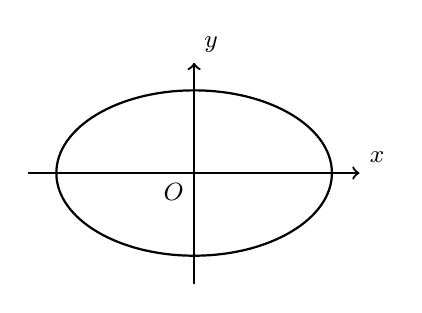
\begin{tikzpicture}[line join = round, line cap = round, thick, font = \small, scale = .7]
\draw[->] (-3,0)--(0,0) node[below left]{$O$}--(3,0) node[above right]{$x$};
\draw[->] (0,-2)--(0,2) node[above right]{$y$};
\draw (0,0) ellipse ({2.5} and {1.5});
\end{tikzpicture}
}
\loigiai{
Hình vẽ trên là của đường elip
}
\end{ex}
%Câu 21
\begin{ex}
Một người có $3$ cái quần khác nhau, $4$ cái áo khác nhau, $2$ cái cà vạt khác nhau. Để chọn một
cái quần hoặc một cái áo hoặc một cái cà vạt thì số cách chọn khác nhau là
\choice
{\True $9$}
{$24$}
{$12$}
{$6$}
\loigiai{
$\bullet $ Nếu chọn một cái quần thì sẽ có $3$ cách.\\
$\bullet $ Nếu chọn một cái áo thì sẽ có $4$ cách.\\
$\bullet $ Nếu chọn một cái cà vạt thì sẽ có $2$ cách.\\
Theo qui tắc cộng, ta có $3+4+2=9$ cách chọn
}
\end{ex}
%Câu 22
\begin{ex}
Ở đậu Hà Lan, $B$ là gene trội quy định tình trạng hạt trơn, $b$ là gene lặn quy định tình trạng hạt
nhăn. Sự tổ hợp giữa hai gene trên tạo ra số kiểu gene là
\choice
{$1$}
{$2$}
{\True $3$}
{$4$}
\loigiai{
Sự tổ hợp giữa gene $B$ và gene $b$ tạo ra các kiểu gene là: BB, Bb, bb.\\
Vậy có 3 kiểu gene
}
\end{ex}
%Câu 23
\begin{ex}
Từ các chữ số $1;2;3;4;5$ có thể lập được bao nhiêu số tự nhiên có 4 chữ số khác nhau?
\choice
{$5$}
{\True $120$}
{$625$}
{$24$}
\loigiai{
Mỗi số có 4 chữ số khác nhau được lập từ các chữ số $1;2;3;4;5$ là một chỉnh hợp chập 4 của 5 phần tử.\\
Số các số tự nhiên có 4 chữ số khác nhau là: $A_5^4=120$(số)
}
\end{ex}
%Câu 24
\begin{ex}
 Số chỉnh hợp chập $3$ của $7$ phần tử bằng
\choice
{\True $210$}
{$35$}
{$6$}
{$5040$}
\loigiai{
Số chỉnh hợp chập $3$ của $7$ phần tử bằng $A_7^3=210$
}
\end{ex}
%Câu 25
\begin{ex}
 Số tổ hợp chập $5$ của $8$ phần tử bằng
\choice
{$6720$}
{\True $56$}
{$120$}
{$40320$}
\loigiai{
Số tổ hợp chập $5$ của $8$ phần tử bằng $C_8^5=56$
}
\end{ex}
%Câu 26
\begin{ex}
 Độ dài của cây cầu người ta đo được là $996m\pm 0{,}5m$. Sai số tương đối tối đa trong phép đo là bao nhiêu?
\choice
{\True $0{,}05\%$}
{$0{,}5\%$}
{$0{,}04\%$}
{$0{,}005\%$}
\loigiai{
Ta có độ dài gần đúng của cầu là $a=996$ với độ chính xác $d=0{,}5$.\\
Vì sai số tuyệt đối $\Delta _a\le d=0{,}5$ nên sai số tương đối $\delta _a=\dfrac{\triangle _a}{|a|}\le \dfrac{d}{|a|}=\dfrac{0{,}5}{996}\approx 0{,}05\%$.\\
Vậy sai số tương đối tối đa trong phép đo trên là $0{,}05\%$
}
\end{ex}
%Câu 27
\begin{ex}
Sản lượng lúa của $40$ thửa ruộng có cùng diện tích được trình bày tròn bảng số liệu sau: 
\begin{center}
\begin{tabular}{|c|c|c|c|c|c|c|}
\hline
Sản lượng & $20$ & $21$ & $22$ & $23$& $24$ & \\
\hline
Tần số & $5$ & $8$ & $11$ & $10$ & $6$ & $N=40$\\
\hline
\end{tabular}
\end{center}
Tính phương sai của bảng số liệu.
\choice
{$1{,}75$}
{\True $1{,}76$}
{$1{,}74$}
{$1{,}73$}
\loigiai{
Ta có $\overline{x}=\dfrac{20 \cdot 5+21 \cdot 8+22 \cdot 11+23 \cdot 10+24 \cdot 6}{40}=22{,}1$\\
$\Rightarrow s^2=\dfrac{1}{40}\left[5{{\left(20-22{,}1\right)}^2}+8{{\left(21-22{,}1\right)}^2}+11{{\left(22-22{,}1\right)}^2}+10{{\left(23-22{,}1\right)}^2}+6{{\left(24-22{,}1\right)}^2}\right]=1{,}76$
}
\end{ex}
%Câu 28
\begin{ex}
Nhiệt độ cao nhất của Hà Nội trong $7$ ngày liên tiếp trong tháng tám được ghi lại là: $34;34;36;35;33;31;30$ (Độ C). Độ lệch chuẩn của mẫu số liệu thuộc khoảng nào dưới đây?
\choice
{\True $\left(1;2\right)$}
{$\left(3;4\right)$}
{$\left[2;\dfrac{7}{2}\right]$}
{$\left(0;\dfrac{3}{4}\right)$}
\loigiai{
Số trung bình cộng của mẫu số liệu là:\\
$\overline{x}=\dfrac{34+34+36+35+33+31+30}{7}\approx 33{,}29$\\
Phương sai của mẫu số liệu là: $s^2=\dfrac{\sum\limits_{i=1}^7 \left(x_i-\overline{x}\right)^2}{7}\approx 3{,}92$\\
Độ lệch chuẩn cần tính là: $s\approx \sqrt{3{,}92}\approx 1{,}98$
}
\end{ex}
%Câu 29
\begin{ex}
Một mẫu số liệu có tứ phân vị thứ nhất là $15$ và tứ phân vị thứ ba là $20$. Giá trị nào sau đây bất thường?
\choice
{$8$}
{$10$}
{$27$}
{\True $28$}
\loigiai{
Ta có $\triangle _Q=20-15=5\Rightarrow $ $Q_1-1{,}5 \cdot \triangle _Q=7{,}5$ và $Q_3+1{,}5 \cdot \triangle _Q=27{,}5$ nên giá trị bất thường là $28$
}
\end{ex}
%Câu 30
\begin{ex}
 Trong một chiếc hộp có $15$ viên bi, trong đó có $6$ viên bi màu đỏ, $5$ viên bi màu xanh và $4$ viên bi màu vàng. Lấy ngẫu nhiên ra 3 viên bi. Tìm xác suất để ba viên bi lấy ra đều có màu xanh?
\choice
{$\dfrac{4}{91}$}
{$\dfrac{4}{455}$}
{$\dfrac{24}{91}$}
{\True $\dfrac{2}{91}$}
\loigiai{ Số phần tử của không gian mẫu: $n\left(\Omega\right)=C_{15}^3$.\\
Gọi $A$ là biến cố: “ba viên bi lấy ra đều có màu xanh”.\\
Số phần tử của biến cố $A$: $n(A)=C_5^3$.\\
Vậy xác xuất của biến cố $A$ là: $P(A)=\dfrac{C_5^3}{C_{15}^3}=\dfrac{2}{91}$
}
\end{ex}
%Câu 31
\begin{ex}
 Một tổ học sinh có $7$ nam và $3$ nữ. Chọn ngẫu nhiên $2$ học sinh tham gia lao động công ích cho nhà trường. Tính xác suất sao cho $2$ học sinh được chọn có ít nhất một học sinh nữ?
\choice
{$\dfrac{7}{15}$}
{\True $\dfrac{8}{15}$}
{$\dfrac{1}{15}$}
{$\dfrac{14}{15}$}
\loigiai{ Số phần tử của không gian mẫu: $n\left(\Omega\right)=C_{10}^2$.\\
Gọi $A$ là biến cố: “hai học sinh được chọn có ít nhất một học sinh nữ”.\\
Số phần tử của biến cố $A$: $n(A)=C_3^1 \cdot C_7^1+C_3^2$.\\
Vậy xác xuất của biến cố $A$ là: $P(A)=\dfrac{C_3^1 \cdot C_7^1+C_3^2}{C_{10}^2}=\dfrac{8}{15}$
}
\end{ex}
%Câu 32
\begin{ex}
 Trong mặt phẳng $Oxy$, cho đường thẳng $d$ có PTTS$\heva{& x=3-2t \\& y=-5+7t}\left(t\in \mathbb{R}\right)$ và điểm $M(2;-4)$. Tính khoảng cách từ điểm $M$ đến đường thẳng $d$?
\choice
{\True $\dfrac{5\sqrt{53}}{53}$}
{$\dfrac{8\sqrt{53}}{53}$}
{$\dfrac{3\sqrt{53}}{53}$}
{$\dfrac{9\sqrt{53}}{53}$}
\loigiai{ Ta có: $\heva{& x=3-2t \\& y=-5+7t}\Leftrightarrow \dfrac{x-3}{-2}=\dfrac{y+5}{7}\Leftrightarrow 7(x-3)=-2(y+5)\Leftrightarrow 7x+2y-11=0$\\
Nên $d\left(M,d\right)=\dfrac{\left| 7 \cdot 2+2 \cdot (-4)-11 \right|}{\sqrt{7^2+2^2}}=\dfrac{5\sqrt{53}}{53}$
}
\end{ex}
%Câu 33
\begin{ex}
Trong mặt phẳng tọa độ $Oxy$, phương trình đường tròn có tâm $I(1;4)$ và đi qua điểm $B(2;6)$ là
\choice
{$(x+1)^2+{{(y+4)}^2}=5$}
{${{(x-1)}^2}+{{(y-4)}^2}=\sqrt{5}$}
{${{(x+1)}^2}+{{(y+4)}^2}=\sqrt{5}$}
{\True ${{(x-1)}^2}+{{(y-4)}^2}=5$}
\loigiai{ Phương trình đường tròn tâm $I(a;b)$ bán kính $R$ có dạng: ${{(x-a)}^2}+{{(y-b)}^2}=R^2$.\\
Ta có: đường tròn có tâm $I(1;4)$ và đi qua điểm $B(2;6)$ nên $R^2=IB^2={{(2-1)}^2}+{{(6-4)}^2}=5$.\\
Khi đó, đường tròn có tâm $I(1;4)$ và bán kính $R^2=5$ có phương trình: ${{(x-1)}^2}+{{(y-4)}^2}=5$
}
\end{ex}
%Câu 34
\begin{ex}
 Phương trình nào sau đây là phương trình chính tắc của đường elip?
\choice
{$\dfrac{x^2}{4}-\dfrac{y^2}{3}=1$}
{$\dfrac{x^2}{4}+\dfrac{y^2}{5}=1$}
{$\dfrac{x^2}{4}+\dfrac{y^2}{7}=1$}
{\True $\dfrac{x^2}{4}+\dfrac{y^2}{3}=1$}
\end{ex}
%Câu 35
\begin{ex}
Cho đường elip có phương trình chính tắc sau: $(E)\colon \dfrac{x^2}{25}+\dfrac{y^2}{9}=1$. Điểm nào sau đây nằm trên đường elip?
\choice
{$A(1;4)$}
{$B(0;4)$}
{\True $C(0;-3)$}
{$D(-1;3)$}
\end{ex}
\noindent{\bf\fontfamily{qag}\selectfont\color{violet}B. PHẦN TỰ LUẬN}
%Câu 36
\begin{ex}
Lập phương trình chính tắc của elip có tâm $O$, hai trục đối xứng là hai trục toạ độ và qua hai điểm $M\left(-2\sqrt{3};\dfrac{3}{2}\right)$, $N\left(2;\dfrac{3\sqrt{3}}{2}\right)$
\loigiai{
Gọi phương trình chính tắc elip cần tìm là $E\colon \dfrac{x^2}{a^2}+\dfrac{y^2}{b^2}=1\left(a>b>0\right)$. Do elip đi qua $M\left(-2\sqrt{3};\dfrac{3}{2}\right)$, $N\left(2;\dfrac{3\sqrt{3}}{2}\right)$ nên ta có hệ $\heva{& \dfrac{12}{a^2}+\dfrac{9}{4b^2}=1 \\& \dfrac{4}{a^2}+\dfrac{27}{4b^2}=1}\Leftrightarrow \heva{& a^2=16 \\& b^2=9}$ \\
Vậy elip cần tìm là $\dfrac{x^2}{16}+\dfrac{y^2}{9}=1$
}
\end{ex}
%Câu 37
\begin{ex}
Đội văn nghệ của nhà trường gồm $4$ học sinh lớp 12A, $3$ học sinh lớp 12B và $2$ học sinh lớp 12C. Chọn ngẫu nhiên 5 học sinh từ đội văn nghệ để biểu diễn trong lễ bế giảng. Hỏi có bao nhiêu cách chọn sao cho lớp nào cũng có học sinh được chọn? 
\loigiai{
Tổng số học sinh trong đội văn nghệ của nhà trường là $9$ học sinh.\\
Số cách chọn $5$ học sinh bất kì trong $9$ học sinh là: $C_9^5$ cách.\\
Số cách chọn $5$ học sinh mà trong đó không có học sinh lớp 12A là: $C_5^5$ cách.\\
Số cách chọn $5$ học sinh mà trong đó không có học sinh lớp 12B là: $C_6^5$ cách.\\
Số cách chọn $5$ học sinh mà trong đó không có học sinh lớp 12C là: $C_7^5$ cách.\\
Vậy có $C_9^5-\left(C_5^5+C_6^5+C_7^5\right)=98$ cách thỏa mãn yêu cầu bài toán
}
\end{ex}

%Câu 38
\begin{ex}
\immini{Nhân dịp nghỉ hè, Minh về quê thăm ông bà ngoại. Nhà ông bà ngoại có một ao cá dạng hình chữ nhật $ABCD$ với chiều dài $BC=20m$, chiều rộng $CD=16m$. Phần tam giác $CEF$ là nơi ông bà nuôi ngan vịt, $BE=5m$, $DF=8m$. Minh đứng ở vị trí $M$ cách $A$ một khoảng $AM=3m$ câu cá và có thể quăng lưỡi câu xa $12{,}5m$. Hỏi lưỡi câu có thể rơi vào khu nuôi vịt của ông bà không?
}{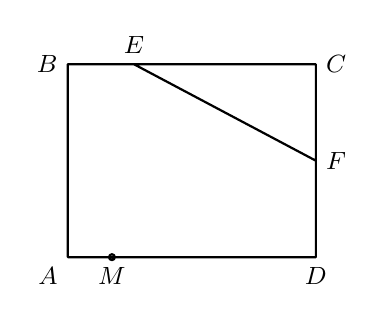
\begin{tikzpicture}[line join = round, line cap = round, thick, font = \small, scale = .7]
\draw (0,0) node[below left]{$A$}--(0.8,0)circle(1.5pt) node[below]{$M$} -- (4.5,0)node[below]{$D$} -- (4.5,1.75)node[right]{$F$}-- (4.5,3.5)node[right]{$C$} -- (1.2,3.5)node[above]{$E$} -- (0,3.5)node[left]{$B$}--(0,0) (4.5,1.75)--(1.2,3.5);
\end{tikzpicture}}
\loigiai{
Chọn hệ trục tọa độ sao cho $A(0;0)$, $M(3;0)$, $E(5;16)$, $F(20;8)$.\\
\begin{center}
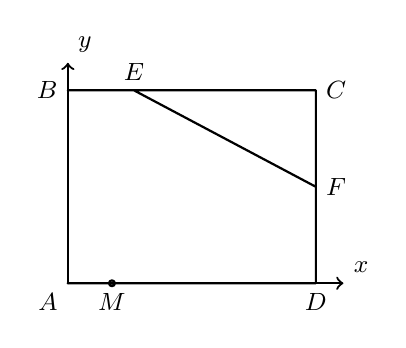
\begin{tikzpicture}[line join = round, line cap = round, thick, font = \small, scale = .7]
\draw[->] (0,0) node[below left]{$A$}--(5,0) node[above right]{$x$};
\draw[->] (0,0)--(0,4) node[above right]{$y$};
\draw (0,0)--(0.8,0)circle(1.5pt) node[below]{$M$} -- (4.5,0)node[below]{$D$} -- (4.5,1.75)node[right]{$F$}-- (4.5,3.5)node[right]{$C$} -- (1.2,3.5)node[above]{$E$} -- (0,3.5)node[left]{$B$} (4.5,1.75)--(1.2,3.5);
\end{tikzpicture}
\end{center}
$\vec{EF}=(15;-8)$\\
Đường thẳng $EF$ đi qua $E(5;16)$ và có một véc tơ pháp tuyến $\vec{n}(8;15)$ nên đường thẳng $EF$ có phương trình: $8(x-5)+15(y-16)=0\Leftrightarrow 8x+15y-280=0$.\\
$d\left(M,EF\right)=\dfrac{\left| 8 \cdot 3+15 \cdot 0-280 \right|}{\sqrt{8^2+{{15}^2}}}=\dfrac{256}{17}\approx 15{,}06$.\\
Do đó Minh không thể quăng lưỡi câu rơi vào khu nuôi ngan vịt
}
\end{ex}
%Câu 39
\begin{ex}
Viết phương trình đường tròn $(C)$ biết đường tròn $(C)$ qua $B(3;1)$ và tiếp xúc với đường thẳng $d\colon 3x-4y-2=0$ tại $A(2;1)$?
\loigiai{
Gọi $I$ là tâm của đường tròn $(C)$\\
Đường thẳng $IA$ qua $A(2;1)$ vuông góc với $d$ có phương trình: $4x+3y-11=0$\\
Gọi $H\left(\dfrac{5}{2};1\right)$ là trung điểm của $AB$. Đường trung trực của $AB$ qua $H$ nhận $\vec{AB}=(1;0)$ là VTPT, khi đó: $IH\colon x-\dfrac{5}{2}=0$\\
Tọa độ tâm $I$ là nghiệm của hệ: $\heva{& x-\dfrac{5}{2}=0 \\& 4x+3y-11=0}\Rightarrow I\left(\dfrac{5}{2};\dfrac{1}{3}\right)\Rightarrow R=IA=\dfrac{5}{6}$\\
Vậy phương trình đường tròn $(C)\colon {{\left(x-\dfrac{5}{2}\right)}^2}+{{\left(y-\dfrac{1}{3}\right)}^2}=\dfrac{25}{36}$
}
\end{ex}

\Closesolutionfile{ans}